\chapter{3D: domain definition and characterization}



\section{Planar domain definition}


\begin{center}
\begin{longtable}{|p {3.5 cm}|p {6.5 cm}|p {3 cm}|p {4 cm}|}
\hline
\textbf{Keyword} & \textbf{Description}  \\ \hline
\endfirsthead
\hline
\multicolumn{4}{| c |}{continued from previous page} \\
\hline
\textbf{Keyword} & \textbf{Description}  \\ \hline
\endhead
\hline
\multicolumn{4}{| c |}{{continued on next page}}\\ 
\hline
\endfoot
\endlastfoot
\hline
DemFile & name of the file providing the DEM map  \\ \hline
LandCoverMapFile & name of the file providing the land cover map  \\ \hline
\caption{Keywords of input file related to the domain}
\label{input_file}
\end{longtable}
\end{center}


\section{Z-coordinate domain definition}

\begin{center}
\begin{longtable}{|p {3.5 cm}|p {4.7 cm}|p {1. cm}|p{0.8 cm}|p{1.4 cm}|p{0.8 cm}|p{1.3 cm}|}
\hline
\textbf{Keyword} & \textbf{Description} & \textbf{M. U.} & \textbf{range} & \textbf{Default Value} & \textbf{Sca / Vec} & \textbf{Str / Num / Opt} \\ \hline
\endfirsthead
\hline
\multicolumn{7}{| c |}{continued from previous page} \\
\hline
\textbf{Keyword} & \textbf{Description} & \textbf{M. U.} & \textbf{range} & \textbf{Default Value} & \textbf{Sca / Vec} & \textbf{Str / Num / Opt} \\ \hline
\endhead
\hline
\multicolumn{7}{| c |}{{continued on next page}}\\ 
\hline
\endfoot
\endlastfoot
\hline
%PointSoilType & Soil type of the simulation point & - &  & NA & vec & num \\ \hline
SoilLayerThicknesses \index{SoilLayerThicknesses} & vector defining the thickness of the various soil layers. If not present, a column of 5 layers 100 mm thick will be assumed & mm &  & 100 & vec & num \\ \hline
SoilLayerNumber \index{SoilLayerNumber} & number of soil layers (is calculated after the number of components of the vector SoilLayerNumber) & - &  & 5 & sca & num \\ \hline
\caption{Keywords of  parameters referred to soil layer}
\label{domain_parameters1D_numeric}
\end{longtable}
\end{center}

\section{Topographical characterization}

\begin{center}
\begin{longtable}{|p {3.5 cm}|p {7 cm}|p {1 cm}|p {1 cm}|}
\hline
\textbf{Keyword} & \textbf{Description}  \\ \hline
\endfirsthead
\hline
\multicolumn{4}{| c |}{continued from previous page} \\
\hline
\textbf{Keyword} & \textbf{Description}  \\ \hline
\endhead
\hline
\multicolumn{4}{| c |}{{continued on next page}}\\ 
\hline
\endfoot
\endlastfoot
\hline
SkyViewFactorMapFile \index{SkyViewFactorMapFile}& name of the file providing the sky view factor map  \\ \hline
SlopeMapFile \index{SlopeMapFile} & name of the file providing the slope steepness map  \\ \hline
RiverNetwork \index{RiverNetwork}& name of the file providing the river network map  \\ \hline
AspectMapFile \index{AspectMapFile} & name of the file providing the aspect map  \\ \hline
CurvaturesMapFile \index{CurvaturesMapFile} & name of the file providing the curvature map  \\ \hline
BedrockDepthMapFile \index{BedrockDepthMapFile}& name of the file providing the bedrock depth map  \\ \hline
\caption{Keywords of input maps necessary to launch the 3D simulation}
\label{table_3D_topochar}
\end{longtable}
\end{center}

\section{Land cover and soil depth characterization}

\begin{center}
\begin{longtable}{|p {3.5 cm}|p {7 cm}|p {1 cm}|p {1 cm}|}
\hline
\textbf{Keyword} & \textbf{Description}  \\ \hline
\endfirsthead
\hline
\multicolumn{4}{| c |}{continued from previous page} \\
\hline
\textbf{Keyword} & \textbf{Description}  \\ \hline
\endhead
\hline
\multicolumn{4}{| c |}{{continued on next page}}\\ 
\hline
\endfoot
\endlastfoot
\hline
LandCoverMapFile \index{LandCoverMapFile} & name of the file providing the land cover map  \\ \hline
SoilMapFile \index{SoilMapFile}& name of the file providing the soil map  \\ \hline
\caption{Keywords of input maps necessary to launch the 3D simulation}
\label{table_3D_landchar}
\end{longtable}
\end{center}



\noindent Each land cover type may be characterized by parameters that define the influence on vegetation, soil surface and snow. Each soil type may be further described in the file {\it PointFile} (see Table \ref{table_3D_landchar_file}) where each row index represents the value corresponding to the {\it SoilMapFile} map.

\begin{center}
\begin{longtable}{|p {2.5 cm}|p {8.5 cm}|p {1 cm}|p {1 cm}|}
\hline
\textbf{Keyword} & \textbf{Description}  \\ \hline
\endfirsthead
\hline
\multicolumn{4}{| c |}{continued from previous page} \\
\hline
\textbf{Keyword} & \textbf{Description}  \\ \hline
\endhead
\hline
\multicolumn{4}{| c |}{{continued on next page}}\\ 
\hline
\endfoot
\endlastfoot
\hline
PointFile \index{PointFile}& name of the file providing the properties for the simulation point  \\ \hline
\caption{Keyword of the file related to the spatial characterization of soil/rock properties. The parameters identified by the row index represent the value corresponding to the SoilMapFile map.}
\label{table_3D_landchar_file}
\end{longtable}
\end{center}

\noindent It is also requested to provide a definition of the average latitude and longitude of the domain area, as specified in Table \ref{topo_par3d_gen}.

\begin{center}
\begin{longtable}{|p {2.3 cm}|p {6. cm}|p {1.5 cm}|p{1.0 cm}|p{1.2 cm}|p{0.8 cm}|p{1. cm}|}
\hline
\textbf{Keyword} & \textbf{Description} & \textbf{M. U.} & \textbf{range} & \textbf{Default Value} & \textbf{Sca / Vec} & \textbf{Log / Num} \\ \hline
\endfirsthead
\hline
\multicolumn{7}{| c |}{continued from previous page} \\
\hline
\textbf{Keyword} & \textbf{Description} & \textbf{M. U.} & \textbf{range} & \textbf{Default Value} & \textbf{Sca / Vec} & \textbf{Log / Num} \\ \hline
\endhead
\hline
\multicolumn{7}{| c |}{{continued on next page}}\\ 
\hline
\endfoot
\endlastfoot
\hline
Latitude \index{Latitude}& Average latitude of the basin, positive means north, negative means south & degree & -90, 90 & 45 & sca & num \\ \hline
Longitude \index{Longitude} & Average longitude of the basin, eastwards from 0 meridiane & degree & 0, 180 & 0 & sca & num \\ \hline
\caption {Keyword of parameters describing the point characterization for 3D simulations}
\label{topo_par3d_gen}
\end{longtable}
\end{center}


\section{Output}

It is possible to define some points where to obtain output information, as described in Par. \ref{par:focusPoints}. The parameters and headers to provide are specified in Table \ref{header_soilrock3D} and \ref{topo_par3d_gen} respectively.


\begin{center}
\begin{longtable}{|p {3.5 cm}|p {4.5 cm}|p {2.5 cm}|p {4 cm}|}
\hline
\textbf{Keyword} & \textbf{Description} & \textbf{Associated file}  \\ \hline
\endfirsthead
\hline
\multicolumn{4}{| c |}{continued from previous page} \\
\hline
\textbf{Keyword} & \textbf{Description} & \textbf{Associated file}  \\ \hline
\endhead
\hline
\multicolumn{4}{| c |}{{continued on next page}}\\ 
\hline
\endfoot
\endlastfoot
\hline
HeaderPointID \index{HeaderPointID}& column name in the file PointFile for the identification ID of the point & PointFile  \\ \hline
HeaderCoordinatePointX \index{HeaderCoordinatePointX} & column name in the file PointFile for the x coordinate of the point & PointFile  \\ \hline
HeaderCoordinatePointY \index{HeaderCoordinatePointY} & column name in the file PointFile for the y coordinate of the point & PointFile  \\ \hline
\caption{Keywords of header that specify the soil/rock spatial characterization for 3D simulation }
\label{header_soilrock3D}
\end{longtable}
\end{center}


\begin{center}
\begin{longtable}{|p {2.2 cm}|p {4.2 cm}|p {2.7 cm}|p{1.0 cm}|p{1.2 cm}|p{0.8 cm}|p{1. cm}|}
\hline
\textbf{Keyword} & \textbf{Description} & \textbf{M. U.} & \textbf{range} & \textbf{Default Value} & \textbf{Sca / Vec} & \textbf{Log / Num} \\ \hline
\endfirsthead
\hline
\multicolumn{7}{| c |}{continued from previous page} \\
\hline
\textbf{Keyword} & \textbf{Description} & \textbf{M. U.} & \textbf{range} & \textbf{Default Value} & \textbf{Sca / Vec} & \textbf{Log / Num} \\ \hline
\endhead
\hline
\multicolumn{7}{| c |}{{continued on next page}}\\ 
\hline
\endfoot
\endlastfoot
\hline
PointID \index{PointID}& identification code for the point of simulation &  &  & NA & vec & num \\ \hline
CoordinatePointX \index{CoordinatePointX} & coordinate X if PixelCoordinates is 1, number of row of the matrix if PixelCoordinates is 0 & m (according to the geographical projection of the maps) &  & NA & vec & num \\ \hline
CoordinatePointY \index{CoordinatePointY}& coordinate Y if PixelCoordinates is 1, number of column of the matrix if PixelCoordinates is 1 & m (according to the geographical projection of the maps) &  & NA & vec & num \\ \hline
\caption{Keywords of point characterization for the choice of point outputs in 3D simulations}
\label{topo_par3d_gen}
\end{longtable}
\end{center}




%\begin{figure}[h!]
%\begin{center}
%  \begin{minipage}[c]{.65\textwidth}
%    \centering
%    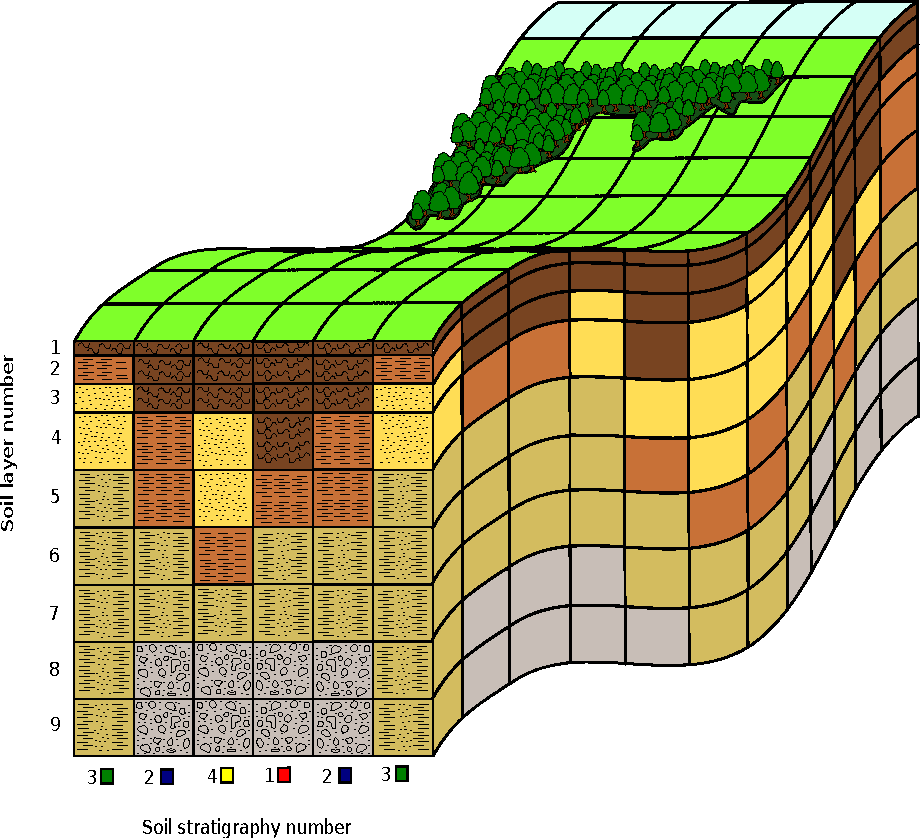
\includegraphics[width=1\textwidth]{./images/pic_spatchar/discretizzazione_3d.pdf}
%  \end{minipage}%
%  \hspace{10mm}%
%  \begin{minipage}[c]{.25\textwidth}
%    \centering
%    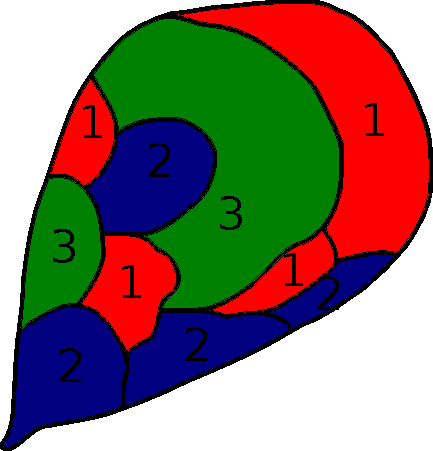
\includegraphics[width=1\textwidth]{./images/pic_spatchar/soil_stratigraphy_basin.pdf}
%  \end{minipage}
%\end{center}
%\textsl{\caption{Soil stratigraphy}\label{ww}}
%\end{figure}


